\documentclass[12pt, a4paper, oneside]{ctexart}
\usepackage[margin=2cm]{geometry}%要先设置页边距,否则页眉页脚会偏
\usepackage{amsmath, amsthm, amssymb, bm, graphicx, hyperref, mathrsfs,float,xcolor,color}
\usepackage{listings}

% 用来设置附录中代码的样式

\lstset{
    basicstyle          =   \bf \ttfamily,          % 基本代码风格
    keywordstyle        =   \bfseries,   % 关键字风格
    keywordstyle        =   \color{blue},
    stringstyle         =   \color{magenta},
    commentstyle        =   \color{red}\ttfamily,
    language            =    [x86masm]Assembler,
    commentstyle        =   \rmfamily\itshape,  % 注释的风格,斜体
    escapeinside=``, % 英文分号中可写入中文
    stringstyle         =   \ttfamily,  % 字符串风格
    columns=fullflexible,%可以自动换行
    breaklines=true,%在单词边界处换行。
    numbers             =   left,   % 行号的位置在左边
    showspaces          =   false,  % 是否显示空格,显示了有点乱,所以不现实了
    numberstyle         =   \zihao{-5}\ttfamily,    % 行号的样式,小五号,tt等宽字体
    showstringspaces    =   false,
    captionpos          =   t,      % 这段代码的名字所呈现的位置,t指的是top上面
    frame               =   lrtb,   % 显示边框
}
\title{实验三 \qquad  简单编程练习}
\author{Leo}
\date{}
\begin{document}
\maketitle
\section{实验任务和实验结果}
% 请写出已通过验收的各个实验任务的具体内容、调试通过的源程序(加注释)和实验结果。
% 实验结果请截图,并加以必要说明。
% 注:按电子版实验三指导,4个基础任务和2个附加任务,实验验收了几个任务,实验报告就相应写几个任务。
\subsection{实验任务1}
在一个数据块中找出最大数。 
假设数据块中的数据为 22、46、32,72、84、16、156,数据块的长度存放在 CX 寄存器中。
\begin{enumerate}
    \item 数据块中的数据为无符号数,找出其中的最大数存放在以 MAXN1 为符号的单元中。
    \item 数据块中的数据为有符号数,找出其中的最大数存放在以 MAXN2 为符号的单元中。 
\end{enumerate} 
\subsubsection{调试通过的源程序}
\begin{lstlisting}
    DATA SEGMENT ;定义数据段
    ARRAY DB 22,46,32,72,84,16,156 ;定义一串数据
    MAXN1 DB 0 ;将存放最大值的变量初始化为0 
    DATA ENDS
    CODE SEGMENT 	;定义代码段
        ASSUME DS:DATA,CS:CODE ;说明代码段、数据段
    START: 
        MOV AX,DATA 
        MOV DS,AX ;给DS赋初值
        MOV CX,6 ;置循环控制数
        LEA DI,ARRAY ;将ARRAY表示的偏移地址送到DI
        MOV DL,[DI] ;将第一个操作数送到寄存器中
        JCXZ LAST 
    AGIN:
        INC DI
        CMP DL,[DI]
        JAE NEXT ;使用无符号数比较指令JAE
        MOV DL,[DI]
    NEXT:
        LOOP AGIN
    LAST:
        MOV MAXN1,DL
        MOV AH,4CH
        INT 21H
    CODE 	ENDS
            END START
\end{lstlisting}
\subsubsection{实验结果}
通过Turbo查看MAXN1相应的内存单元(DS:0007),发现其存储的内容是9C,即无符号数156,说明已经将最大数存到指定位置。
\begin{figure}[H]
    \centering
    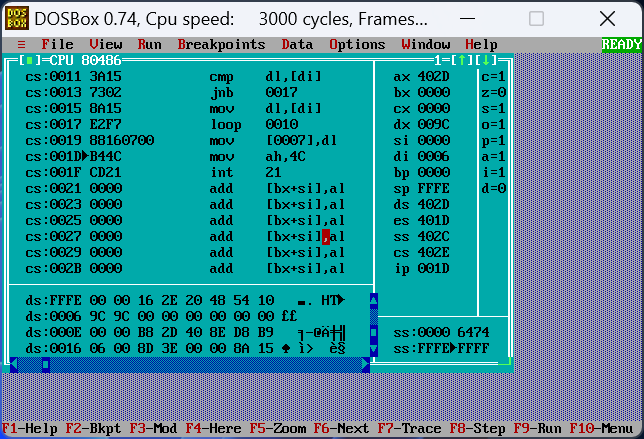
\includegraphics[scale=0.6]{pic/exp1_1_outcome.png}
    \caption{实验1(第一部分)结果截图}
\end{figure}
接下来是有符号数的比较
\begin{lstlisting}
    DATA SEGMENT ;定义数据段
    ARRAY DB 22,46,32,72,84,16,156 ;定义一串数据
    MAXN1 DB 0 ;将存放最大值的变量初始化为0 
    DATA ENDS
    CODE SEGMENT 	;定义代码段
        ASSUME DS:DATA,CS:CODE ;说明代码段、数据段
    START: 
        MOV AX,DATA 
        MOV DS,AX ;给DS赋初值
        MOV CX,6 ;置循环控制数
        LEA DI,ARRAY ;将ARRAY表示的偏移地址送到DI
        MOV DL,[DI] ;将第一个操作数送到寄存器中
        JCXZ LAST 
    AGIN:
        INC DI
        CMP DL,[DI]
        JGE NEXT ;带符号数比较,DL>[DI]时跳转,跳过更新环节
        MOV DL,[DI]
    NEXT:
        LOOP AGIN
    LAST:
        MOV MAXN1,DL
        MOV AH,4CH
        INT 21H
    CODE 	ENDS
            END START
\end{lstlisting}
\subsubsection{实验结果}
通过Turbo查看MAXN1相应的内存单元(DS:0007),发现其存储的内容是54,即有符号数84,说明已经将最大数存到指定位置。
\begin{figure}[H]
    \centering
    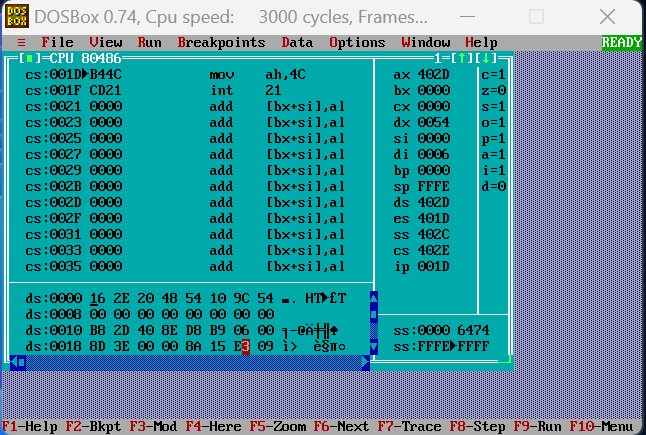
\includegraphics[scale=1]{pic/exp1_2.png}
    \caption{实验1(第二部分)结果截图}
\end{figure}
\subsection{实验任务3}
\subsubsection{实验任务的具体内容}
求无符号字节数据之和,和数为 16 位二进制数。假设有数据 58、25,45,73、64,43,数据块的长度存放在 CX 寄存器中,和数存放在以 SUM 为符号
的字单元中。 
\subsubsection{调试通过的源程序}
\begin{lstlisting}
    DATA SEGMENT ;定义数据段
    ARRAY DW 58,25,45,73,64,43 ;定义一串数据
    SUM DW 0 ;将存放最大值的变量初始化为0 
    DATA ENDS
    CODE SEGMENT 
    ASSUME DS:DATA,CS:CODE ;说明代码段、数据段
    START: 
        MOV AX,DATA 
        MOV DS,AX ;给DS赋初值
        MOV AX,0;
        MOV CX,6
        LEA DI,ARRAY ;将ARRAY表示的偏移地址送到DI
    AGIN:
        ADD AX,[DI];刚开始没加方框
        INC DI
        INC DI
        LOOP AGIN ;该条指令执行后CX自动-1,手动写反而出错
    LAST:
        MOV SUM,AX
        MOV AH,4CH
        INT 21H
    CODE 	ENDS
            END START
    ;当以CX=1状态来到LOOP时,LOOP不会继续循环,而是将CX-1然后跳出循环
\end{lstlisting}
\subsubsection{实验结果}
因为每个数为16位(2Byte),所以和数SUM的内存单元偏移地址为000CH和000DH两个字节。查看该内存单元内容,如图所示为0134H,经检验,计算正确。
\begin{figure}[H]
    \centering
    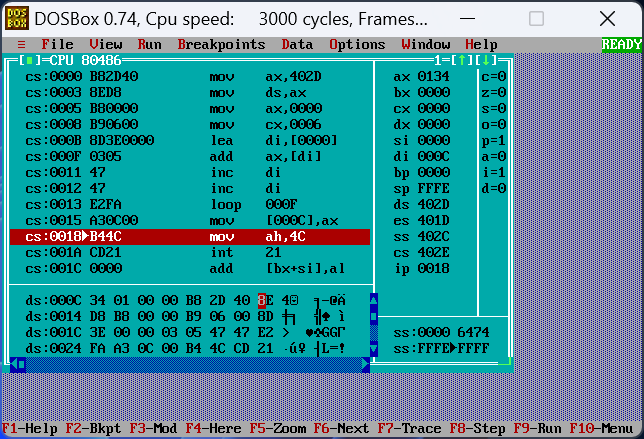
\includegraphics[scale=0.6]{pic/exp1_3.png}
    \caption{实验3结果截图}
\end{figure}
\subsection{实验任务4}
\subsubsection{实验任务的具体内容}
求两个十进制数相乘的积(56093×5 = ?)改为(53348×9 =?),被乘数和乘数均以非压缩 BCD 码表
示,并存放在内存中,乘积以非压缩 BCD 码的格式存放在以 SUM 为起始符号的单元中。
\subsubsection{调试通过的源程序}
\begin{lstlisting}
    DATA SEGMENT ;定义数据段
    D1 DB 08,04,03,03,05
    D2 DB 09 ;这两个十进制数相乘,不超过6位
    SUM DB 6 DUP(0) ;将存放最大值的变量初始化为0,预先不知道结果多长,但是不会超过6位
    DATA ENDS
    CODE SEGMENT 
    ASSUME DS:DATA,CS:CODE ;说明代码段、数据段
    GO: 
        MOV AX,DATA 
        MOV DS,AX ;给DS赋初值
        MOV SI,OFFSET D1 
        MOV BL,[D2];;把乘数放入BL
        MOV DI,OFFSET SUM ;目标存放地址放入DI
        MOV DX,0;因后续进位存放在DL,先清零
        MOV CX,5 ;做乘法的次数,设置为SUM单元的长度
    NEXT:
        MOV AL,[SI] ;将被乘数从低位移入
        INC SI
        MUL BL
        AAM;乘法的ASCII调整,AX中存放非压缩乘积,乘积的低位在AL,高位在AH
        ADD AL,DL ;加上进位
        AAA ;作加法的ASCII调整,把可能的进位加到AH上
        MOV DL,AH;低位向高位的进位要留起来
        MOV [DI],AL ;低位存入目的存储单元
        INC DI
        LOOP NEXT
        MOV [DI],AH
        MOV AH,4CH
        INT 21H
    CODE 	ENDS
            END GO
\end{lstlisting}
\subsubsection{实验结果}
一个5位数乘以一个1位数,结果的长度不会超过6位,所以预先将答案对应的内存单元预置为6Byte。存乘数时,低位排在前面,高位排在后面,从低位开始,每做一次乘法,都做一次ASCII调整,本位存入内存单元,进位暂时放在寄存器,作为下一次乘法的进位。最高位都做完乘法之后,也存入存储单元。结果如图
\begin{figure}[H]
    \centering
    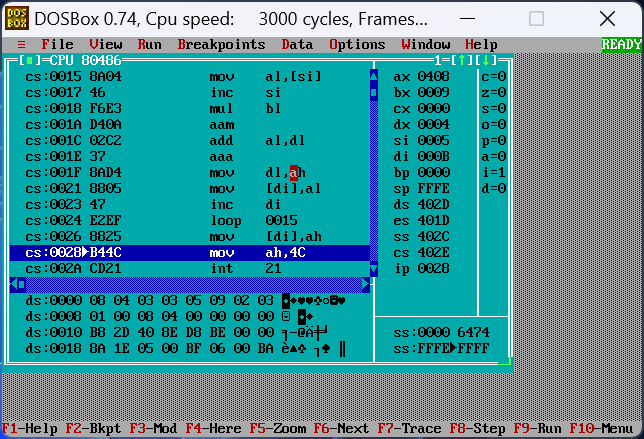
\includegraphics[scale=0.6]{pic/exp1_4.png}
    \caption{实验4结果截图}
\end{figure}
结果的存储位置从ds:0006H开始,到ds:000BH结束。低位排在前面,每一位都是非压缩的BCD码。计算结果为480132,经检验,计算正确。
\subsection{实验任务5}
\subsubsection{实验任务的具体内容}
请用串传送指令编写程序,将以 STR1 为首地址的字节存储单元中的数据 30H、31H,32H、33H,34H、
35H、36H、37H、38H,39H、40H、41H,42H,43H,44H、45H,传送到以 STR2 为首地址的字节存储单元中。
\subsubsection{调试通过的源程序}
\begin{lstlisting}
    DATA SEGMENT ;定义数据段
    STR1 DB 30H,31H,32H,33H,34H,35H,36H,37H,38H,39H,40H,41H,42H,43H,44H,45H
    STR2 DB 16 DUP(?) 
    DATA ENDS
    CODE SEGMENT 
    ASSUME DS:DATA,CS:CODE ;说明代码段、数据段
    GO: 
    MOV AX,DATA 
        MOV DS,AX ;给DS赋初值
        MOV ES,AX ;给ES赋初值
        MOV SI,OFFSET STR1 
        MOV DI,OFFSET STR2
        MOV CX,16
        CLD
        REP MOVSB
        MOV AH,4CH
        INT 21H
    CODE 	ENDS
            END GO
\end{lstlisting}
\subsubsection{实验结果}
数据串的每一个数据都是Byte为单位,所以用MOVSB指令。查看内存单元ds:0010H到ds:0020H,可以看到数据串已经全部传送到指定位置
\begin{figure}[H]
    \centering
    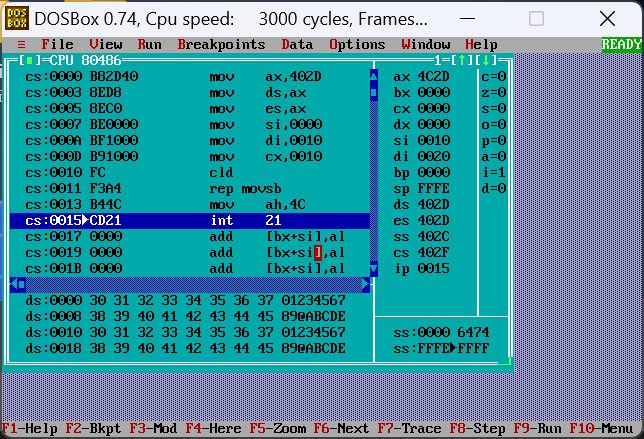
\includegraphics[scale=0.6]{pic/exp1_5.png}
    \caption{实验4结果截图}
\end{figure}

\subsection{实验任务6}
\subsubsection{实验任务的具体内容}
将任务4的乘积在屏幕上显示出来。
\subsubsection{调试通过的源程序}
\begin{lstlisting}
    DATA SEGMENT ;定义数据段
    D1 DB 08,04,03,03,05
    D2 DB 09 ;这两个十进制数相乘,不超过6位
    SUM DB 6 DUP(0) ;将存放最大值的变量初始化为0,预先不知道结果多长
    OTHER DB 0DH,0AH,'$' ;为了使用字符串输出指令,加上回车、换行和$
    DATA ENDS
    CODE SEGMENT 
    ASSUME DS:DATA,CS:CODE ;说明代码段、数据段
    GO: 
        MOV AX,DATA 
        MOV DS,AX ;给DS赋初值
        MOV SI,OFFSET D1 
        MOV BL,[D2];把乘数放入BL
        MOV DI,OFFSET OTHER ;目标存放地址放入DI
        DEC DI;指到SUM单元的最后一位,低位放后面,便于后续正序输出
        MOV DX,0;因后续进位存放在DL,先清零
        MOV CX,5 ;做乘法的次数
    NEXT:
        MOV AL,[SI] ;将被乘数从低位移入
        INC SI
        MUL BL
        AAM;乘法的ASCII调整,AX中存放非压缩乘积,乘积的低位在AL,高位在AH
        ADD AL,DL ;加上进位
        AAA ;作加法的ASCII调整,把可能的进位加到AH上
        MOV DL,AH;低位向高位的进位要留起来
        ADD AL,30H;ASCII数字字符的范围是30H(0)~39H(9)
        MOV [DI],AL ;低位存入目的存储单元
        DEC DI
        LOOP NEXT
        ADD AH,30H;这时候已经是最后的高位了,要加30H来从非压缩BCD码转换到ASCII码
        MOV [DI],AH;此时DI已经指到最高位
        CMP AH,30H
        JNE LAST
        INC DI ;若最高位为0.从次高位开始输出(结果要么是5位要么是6位)
    LAST:
        MOV DX,DI; 字符串的首址放到DX,准备输出
        MOV AH,9 ;调用输出字符串的功能
        INT 21H;输出字符串
        MOV AH,4CH
        INT 21H
    CODE 	ENDS
            END GO
\end{lstlisting}
\subsubsection{实验结果}
左图是在Turbo Debugger中的结果。查看内存单元ds:0006H到ds:000BH,发现所有数字都转换为ASCII字符存储在单元中。在程序中调用打印字符串的中断服务,在DOS中可以看到,计算结果480132已经输出在屏幕上。
\begin{figure}[H]
    \centering
    \begin{minipage}{0.45\textwidth}
    \centering
    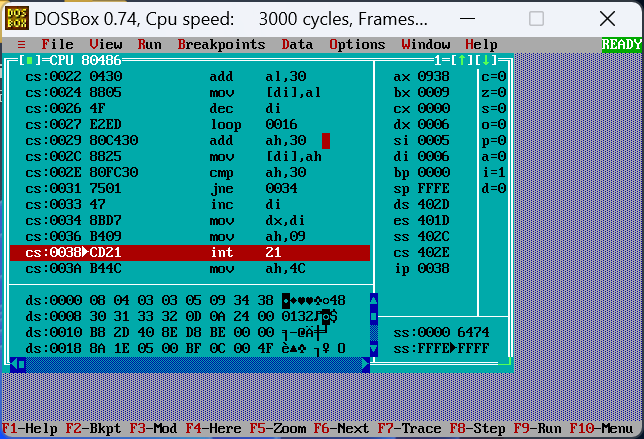
\includegraphics[scale=0.35]{pic/exp1_6_1.png}
    \caption{实验6结果截图1}
    \end{minipage}
    \hspace{0.05\textwidth}
    \begin{minipage}{0.45\textwidth}
    \centering
    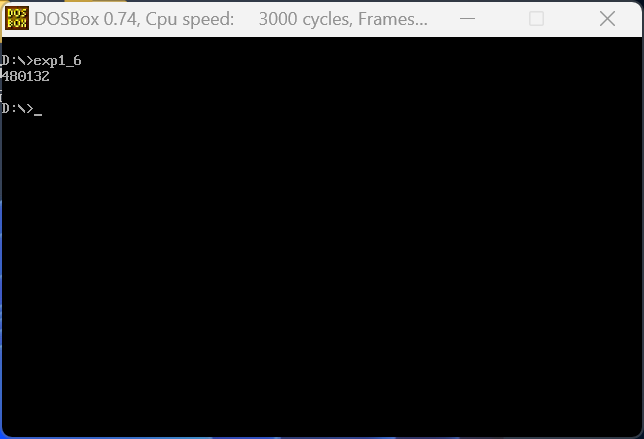
\includegraphics[scale=0.35]{pic/exp1_6_2.png}
    \caption{实验6结果截图2}
    \end{minipage}
\end{figure}
\subsection{实验任务7}
\subsubsection{实验任务的具体内容}
在数据段和附加数据段中各定义一个 10 字节的字符串,请编程比较这两个字符串是否完全相同。
 若两串完全相同,则将数据段中存放比较结果的 RESULT1 单元赋值为 0; 
 若两串不同,则将源串中第 1 个不相同字节的地址赋给数据段中的 RESULT1 单元,并将该字节内
容送到数据段中的RESULT2单元。
\subsubsection{调试通过的源程序}
\begin{lstlisting}
    ;第一次实验:两串不相同。第二次实验,把STR2改为'HELLO12345',两串相同
    DATA SEGMENT ;定义数据段
    STR1 DB 'HELLO12345'
    RESULT1 DB 0
    RESULT2 DB 0
    DATA ENDS
    EXTRA SEGMENT;定义附加段
    STR2 DB 'HELLO1?345' ;两串不完全相同
    EXTRA ENDS
    CODE SEGMENT 
    ASSUME DS:DATA,CS:CODE,ES:EXTRA ;说明代码段、数据段
    GO: 
        MOV CX,10
        MOV AX,DATA 
        MOV DS,AX ;给DS赋初值
        MOV AX,EXTRA
        MOV ES,AX;给ES赋初值
        MOV SI,OFFSET STR1;
        MOV DI,OFFSET STR2
        REPE CMPSB
        JZ EQQ;若不完全一样,就不跳转
        DEC SI;恢复到不一样的地方
        MOV BX,SI;传送相异字节所在的地址
        MOV [RESULT1],BL ;只有变量才可以用LOW指令
        MOV AL,[SI]
        MOV [RESULT2],AL
        JMP LAST
    EQQ: 
        MOV [RESULT1],0;若完全相同,RESULT1置0
    LAST:
        MOV AH,4CH
        INT 21H
    CODE 	ENDS
            END GO
\end{lstlisting}
\subsubsection{实验结果}
第一次实验的结果如图所示,图\ref{实验7结果截图1}和图\ref{实验7结果截图2}展示的是ES段和DS段的数据,表明目的串与源串不同。图\ref{实验7结果截图2}显示了DS段的数据。从ds:0000H到ds:0009H存的是源串。ds:000AH存的是RESULT1,存放了第一个字符不一致的地址,即06;ds:000BH存的是RESULT2,存放了源串中这个不一样的字符,即'2'。
\begin{figure}[H]
    \centering
    \begin{minipage}{0.45\textwidth}
    \centering
    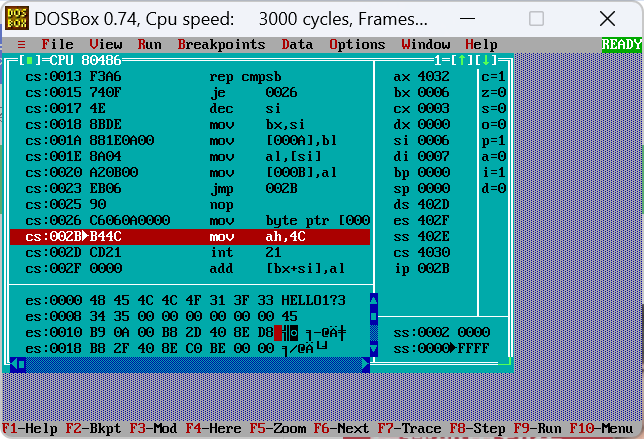
\includegraphics[scale=0.35]{pic/exp1_7_1es_segment.png}
    \caption{实验7结果截图1}
    \label{实验7结果截图1}
    \end{minipage}
    \hspace{0.05\textwidth}
    \begin{minipage}{0.45\textwidth}
    \centering
    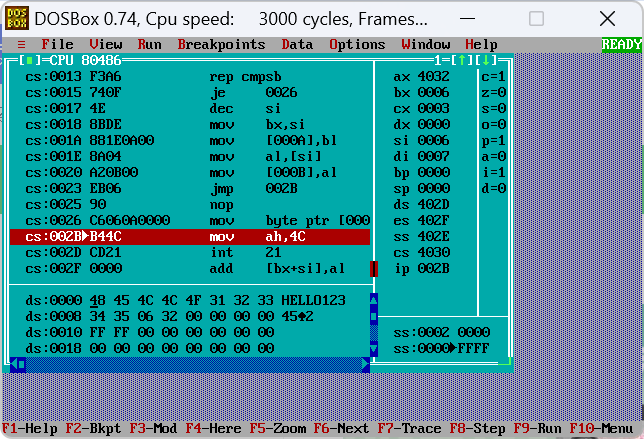
\includegraphics[scale=0.35]{pic/exp1_7_1unequal.png}
    \caption{实验7结果截图2}
    \label{实验7结果截图2}
    \end{minipage}
\end{figure}
第二次实验,将两个字符串的内容设为一致,都为'HELLO12345',结果如图\ref{实验7结果截图3}、图\ref{实验7结果截图4},从后者可以看到,RESULT1中存放的数据为00H,说明比较结果为两字符串相同。
\begin{figure}[H]
    \centering
    \begin{minipage}{0.45\textwidth}
    \centering
    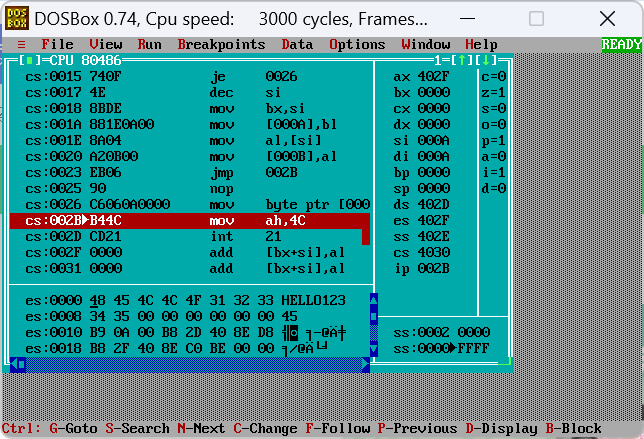
\includegraphics[scale=0.35]{pic/exp1_7_2es_segment.png}
    \caption{实验7结果截图3}
    \label{实验7结果截图3}
    \end{minipage}
    \hspace{0.05\textwidth}
    \begin{minipage}{0.45\textwidth}
    \centering
    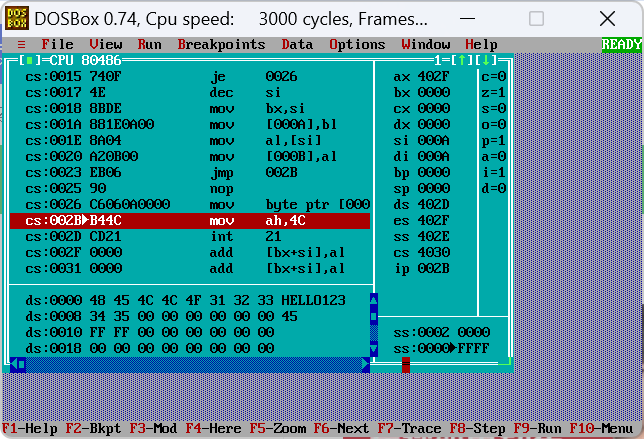
\includegraphics[scale=0.35]{pic/exp1_7_2equal.png}
    \caption{实验7结果截图4}
    \label{实验7结果截图4}
    \end{minipage}
\end{figure}
\section{实验总结}
\begin{enumerate}
    \item 实验1刚开始用字作为单位存储,但每次INC只一次,导致出错。后来发现可以用字节存储。
    \item 将变量的地址装入寄存器时容易忘写OFFSET
    \item 实验3使用MOV CX,(LENGTH DATA)-1 ;置循环控制数。报错must be associated with data。后来选择用立即数置数解决
    \item 实验3用到LOOP指令,该条指令执行后CX自动-1,手动减少CX的值反而会出错
    \item 实验4:预先不知道计算结果多长的时候可以先置足够大的空间备用。(在该环境下,对没有用DUP定义的单元都认为LENGTH=1?)
    \item 定义字符串时注意全角/半角和中英文引号的区别
    \item 实验6打印时刚开始总打印乱码。后来发现要将数字转化为16进制下的ASCII码才能正确打印。对非压缩BCD码,调整为ASCII只需要加30H
    \item 实验7最开始总是指不到不一样的那个字符。后来发现由于CMPSB指令使SI自增,因此找到相异处之后要将SI-1才指到不一样的那个字符
\end{enumerate}
% 如,上述实验任务的程序调试中遇到什么错误或问题,是如何查找、改正程序错误或如何解决问题的。
\section{思考题}
\begin{enumerate}
    \item CMP BL,00用于检查BL存的内容是否为00H,可以用SUB BL,00代替。
    \item 前者用JA/JNBE等,后者用JGE/JNLE等
    \item 源操作数用的是间接寻址方式。可以用MOV AX,NUM MOV SI,AX两条指令代替
    \item 用了AAM和AAA指令。调整方法:对于AAA,若二进制数计算结果的低4位大于9或发生进位(AF=1),则要加上0110调整。若高四位大于9或发生进位(CF=1),也要加0110调整。对于AAM,将AL的值除以10H,结果放入AH,AL对10H取余,结果放在AL。第一次执行AAM后AX=0702H(十进制下8*9=72),第一次执行AAA后AX=0403H(十进制下4*9+7=43)
    \item DF用于控制串操作指令中,SI和DI是自增还是自减。用CLD置0,表示自增;用STD置1,表示自减.
\end{enumerate}
% 请按电子版实验三指导,第1个思考题必答,后面五个附加思考题可选择回答部分问题或全部问题。

\end{document}